\newif \ifshare
% \sharetrue % Comment this if you want animation
\ifshare % "Share mode" without animation.
\documentclass[table, trans, aspectratio = 169]{beamer}
\else % "Presentation mode" with animation.
\documentclass[table, aspectratio = 169]{beamer}
\fi
\usepackage{default}
\usepackage[T1]{fontenc}
\usepackage{color}
\usepackage{graphicx}
\usepackage{subfig}
\usepackage{diagbox}


\let\pgfmathMod=\pgfmathmod\relax

\graphicspath{{../figs/PDF/}}

\usetheme{Boadilla}

\definecolor{struct}{HTML}{03a9f4}
\definecolor{alert}{HTML}{f44336}
\definecolor{example}{HTML}{aeea00}
\definecolor{good}{HTML}{8bc34a}
\definecolor{notgoodnotbad}{HTML}{ff9800}

\setbeamercolor{structure}{fg = struct}
\setbeamercolor{normal text}{fg = white, bg = black}
\setbeamercolor{example text}{fg = example}
\setbeamercolor{alerted text}{fg = alert}
\setbeamercolor{footline}{fg = white}

\title[FOSDEM 2023]{Inspektor Gadget: An eBPF Based Tool to Observe Containers}
\subtitle{FOSDEM 2023}
\author[Francis Laniel (\texttt{flaniel@linux.microsoft.com})]{Francis Laniel\\\texttt{flaniel@linux.microsoft.com}}
\date{5th February 2023}

% Custom title page.
\defbeamertemplate*{title page}{customized}[1][]{
	\centering
	\usebeamerfont{title}\usebeamercolor[fg]{title}\inserttitle\par
	\usebeamerfont{subtitle}\usebeamercolor[fg]{subtitle}\insertsubtitle\par
	\bigskip
	\usebeamerfont{author}\usebeamercolor[fg]{normal text}\textbf{\insertauthor}\par
	\bigskip
	\usebeamerfont{date}\usebeamercolor[fg]{normal text}\textbf{\insertdate}\par
	\bigskip
	\bigskip

	\begin{columns}
		\begin{column}{.5\textwidth}
			\centering

			\includegraphics[scale=2]{microsoft.pdf}
		\end{column}
		\begin{column}{.5\textwidth}
			\centering

			\includegraphics{kinvolk.pdf}
		\end{column}
	\end{columns}
}

\begin{document}
	% Put these parameters here to avoid compilation error:
	% "! LaTeX Error: Missing \begin{document}."
	% Remove the navigation bar, this is useless...
	\setbeamertemplate{navigation symbols}{}
	% Use square instead of bubbles, see:
	% https://tex.stackexchange.com/a/69721
	\setbeamertemplate{section in toc}[square]
	% Modify the shaded value to 60% instead of 20%, see:
	% https://tex.stackexchange.com/a/66703
	\setbeamertemplate{sections/subsections in toc shaded}[default][50]
	% Use circle instead of bubbles for itemize, see:
	% \setbeamertemplate{itemize items}[circle]
	\setbeamertemplate{itemize items}[square]
	\setbeamertemplate{enumerate items}[square]

	\maketitle

	\section{Introduction}
	\begin{frame}
		\frametitle{The containers}

		\begin{columns}
			\begin{column}{.5\textwidth}
				The containers rely on several features offered by the kernel:
				\begin{description}
					\item[The \texttt{namespaces}:] Security isolation \cite{rami_rosen_namespace_2016, kerrisk_lce_2012, kerrisk_namespaces_2013}.
					\item[The \texttt{cgroups}:] Resources isolation \cite{rami_rosen_namespace_2016, hiroyu_cgroup_2008}.
				\end{description}
			\end{column}
			\begin{column}{.5\textwidth}
				\centering

				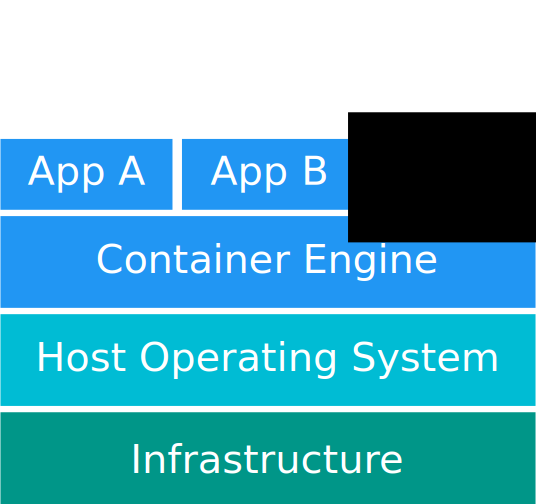
\includegraphics[scale = .42]{container.pdf}

				Container (\texttt{docker}, \texttt{lxc}, \texttt{podman}, etc.)
			\end{column}
		\end{columns}
	\end{frame}

	\section{Problem}
	\begin{frame}
		\frametitle{Containers can be hard to debug}

		Using containers pose several problems to debug applications, among others:
		\begin{itemize}
			\item Harder to attach a debugger to running application.
			\item One have to take into account the communications between different containers.
		\end{itemize}
	\end{frame}

	\section{Inspektor Gadget}
	\begin{frame}
		\frametitle{Inspektor Gadget}
		\framesubtitle{Presentation}

		\begin{columns}
			\begin{column}{.3\textwidth}
				\centering

				\includegraphics[scale=.33]{inspektor_gadget.pdf}%

				A swiss army knife based on eBPF \cite{inspektor_gadget_contributors_inspektor_nodate}:
				\begin{itemize}
					\item \texttt{local-gadget}
					\item \texttt{kubectl-gadget}
				\end{itemize}
			\end{column}
			\begin{column}{.7\textwidth}
				\centering

				\includegraphics<1>[scale=.2]{inspektor_gadget_tools-fig1.pdf}%
				\includegraphics<2>[scale=.2]{inspektor_gadget_tools-fig2.pdf}%
				\includegraphics<3>[scale=.2]{inspektor_gadget_tools-fig3.pdf}%
				\includegraphics<4>[scale=.2]{inspektor_gadget_tools-fig4.pdf}%
				\includegraphics<5>[scale=.2]{inspektor_gadget_tools-fig5.pdf}%
				\includegraphics<6>[scale=.2]{inspektor_gadget_tools-fig6.pdf}%

				The different tools offered by Inspektor Gadget.
			\end{column}
		\end{columns}
	\end{frame}

	\begin{frame}
		\frametitle{Inspektor Gadget}
		\framesubtitle{Short demo}

		Comparing \texttt{local-gadget trace exec} to \texttt{execsnoop} \cite{iovisorbcc_contributors_execsnoop_nodate}.
	\end{frame}

	\begin{frame}
		\frametitle{Inspektor Gadget}
		\framesubtitle{What is eBPF?}

		According to Brendan Gregg \cite{gregg_learn_2019}:
		\begin{quote}
			eBPF does to Linux what JavaScript does to HTML.
			[...]
			[W]ith eBPF, instead of a fixed kernel, you can now write mini programs that run on events like disk I/O, which are run in a safe virtual machine in the kernel.
		\end{quote}

		\bigskip

		\onslide<2>{
			eBPF programs safety comes with some limitations, among others:
			\begin{itemize}
				\item It is impossible to write an infinite or a not statically bounded loop.
				\item There is no function like \texttt{malloc}.
			\end{itemize}
		}
	\end{frame}

	\begin{frame}
		\frametitle{Inspektor Gadget}
		\framesubtitle{eBPF in the Linux kernel}

		\centering

		\includegraphics<1>[scale=.5]{kernel_ebpf-fig1.pdf}%
		\includegraphics<2>[scale=.5]{kernel_ebpf-fig2.pdf}%
		\includegraphics<3>[scale=.5]{kernel_ebpf-fig3.pdf}%
		\includegraphics<4>[scale=.5]{kernel_ebpf-fig4.pdf}%

		Development, loading and execution of an eBPF program \cite{ebpf_contributors_what_nodate}.
	\end{frame}

	\begin{frame}
		\frametitle{Inspektor Gadget}
		\framesubtitle{Internal architecture of \texttt{local-gadget}}

		\centering

		\includegraphics<1>[scale=.5]{local_gadget_manager-fig1.pdf}%
		\includegraphics<2>[scale=.5]{local_gadget_manager-fig2.pdf}%
		\includegraphics<3>[scale=.5]{local_gadget_manager-fig3.pdf}%
		\includegraphics<4>[scale=.5]{local_gadget_manager-fig4.pdf}%
		\includegraphics<5>[scale=.5]{local_gadget_manager-fig5.pdf}%
	\end{frame}

	\begin{frame}
		\frametitle{Inspektor Gadget}
		\framesubtitle{Real world demonstration of \texttt{local-gadget}}

		How to use \texttt{local-gadget} to verify \texttt{seccomp} profile?
	\end{frame}

	\begin{frame}
		\frametitle{Inspektor Gadget}
		\framesubtitle{In Kubernetes}

		\centering

		\includegraphics<1>[scale=.5]{inspektor_gadget_k8s-fig1.pdf}%
		\includegraphics<2>[scale=.5]{inspektor_gadget_k8s-fig2.pdf}%
		\includegraphics<3>[scale=.5]{inspektor_gadget_k8s-fig3.pdf}%
		\includegraphics<4>[scale=.5]{inspektor_gadget_k8s-fig4.pdf}%
		\includegraphics<5>[scale=.5]{inspektor_gadget_k8s-fig5.pdf}%
		\includegraphics<6>[scale=.5]{inspektor_gadget_k8s-fig6.pdf}%
		\includegraphics<7>[scale=.5]{inspektor_gadget_k8s-fig7.pdf}%
		\includegraphics<8>[scale=.5]{inspektor_gadget_k8s-fig8.pdf}%
		\includegraphics<9>[scale=.5]{inspektor_gadget_k8s-fig9.pdf}%
	\end{frame}

	\begin{frame}
		\frametitle{Inspektor Gadget}
		\framesubtitle{Real world demonstration of \texttt{kubectl-gadget}}

		How to use \texttt{kubectl-gadget} to verify the containers \texttt{capabilities}?
	\end{frame}

	\section{Conclusion}
	\begin{frame}
		\frametitle{Conclusion and future works}

		Conclusion:
		\begin{enumerate}
			\item Inspektor Gadget permits monitoring of containers.
			\item It is of precious help to debug these applications.
		\end{enumerate}

		\bigskip

		\onslide<2->{
			Future works:
			\begin{enumerate}
				\item Improve scaling.
				\item Addition of new gadgets.
			\end{enumerate}
		}

		\bigskip

		\onslide<3->{
			Where to find us:
			\begin{itemize}
				\item[{
\includegraphics[scale=.08]{inspektor_gadget_arrow.pdf}}]  \texttt{inspektor-gadget.io}
				\item[{\includegraphics[scale=.01]{github.pdf}}]  \texttt{github.com/inspektor-gadget/inspektor-gadget}
				\item[{\includegraphics[scale=.08]{slack.pdf}}]  \texttt{\#inspektor-gadget (k8s slack)}
			\end{itemize}
		}
	\end{frame}

	\begin{frame}[allowframebreaks, noframenumbering]
		\frametitle{Bibliographie}
		\setbeamertemplate{bibliography item}[text]

		\begin{scriptsize}
			\bibliographystyle{IEEEtran}
			\bibliography{beamer}
		\end{scriptsize}
	\end{frame}
\end{document}
